%%%%%%%%%%%%%%%%%%%%%%%%%%%%%%%%%%%%%%%%%
% University/School Laboratory Report
% LaTeX Template
% Version 3.1 (25/3/14)
%
% This template has been downloaded from:
% http://www.LaTeXTemplates.com
%
% Original author:
% Linux and Unix Users Group at Virginia Tech Wiki 
% (https://vtluug.org/wiki/Example_LaTeX_chem_lab_report)
%
% License:
% CC BY-NC-SA 3.0 (http://creativecommons.org/licenses/by-nc-sa/3.0/)
%
%%%%%%%%%%%%%%%%%%%%%%%%%%%%%%%%%%%%%%%%%

%----------------------------------------------------------------------------------------
%	PACKAGES AND DOCUMENT CONFIGURATIONS
%----------------------------------------------------------------------------------------

\documentclass{article}

\usepackage{graphicx} % Required for the inclusion of images
\usepackage{natbib} % Required to change bibliography style to APA
\usepackage{amsmath} % Required for some math elements 
\usepackage{amsthm}
\usepackage[hyphens]{url}
\usepackage{hyperref}
\usepackage{subcaption}
\usepackage{float}
\usepackage{array}
\usepackage{amssymb}


\setlength\parindent{0pt} % Removes all indentation from paragraphs

\newtheorem*{remark}{Theorem}
\newtheorem*{definition}{Definition}

%----------------------------------------------------------------------------------------
%	DOCUMENT INFORMATION
%----------------------------------------------------------------------------------------

\title{Homework \#3 \\RSA \\[0.2em]\small{}CNS Course Sapienza} % Title and subtitle

\author{Riccardo \textsc{Prinzivalle}, 1904064} % Author name

\date{November 20, 2020} % Date for the report

\begin{document}

\maketitle % Insert the title, author and date

%----------------------------------------------------------------------------------------
%	SECTION 0
%----------------------------------------------------------------------------------------

\section{Homework Goal}

This homework contains an implementation of RSA algorithm based on major libraries for the mathematical functions, a comparison with the insecure \textit{PyCryptoDome} RSA and with the \textit{PyCryptoDome} AES.

%----------------------------------------------------------------------------------------
%	SECTION 1
%----------------------------------------------------------------------------------------

\section{RSA Implementation}

RSA algorithm is basically divided in two part: the initialization and the encryption. The encryption phase is simpler than the initialization: it uses only an exponentiation and a modulo reduction. The modulo reduction is already implemented in python (used in this homework), instead what it is needed is an efficient implementation of the exponentiation. To do so, I used the proposed \textbf{Square And Multiply} in the slides of the course: at first with small values of base and exponent it worked flawlessly, but during the test with bigger messages and keys, the computation explodes, so I thought to reduce in modulo after every performed computation (since we have to do it after the exponentiation, so why don't do it at every step?) and the \textbf{SAM} computation time dropped to some seconds. The code can be seen in Fig. \ref{fig:sam}

\begin{figure}[H]
	\centering
	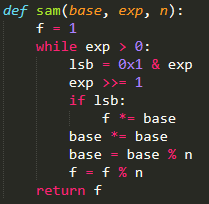
\includegraphics[width=0.345\linewidth]{images/SAM.png}
	\caption{Improved version of Square And Multiply}
	\label{fig:sam}
\end{figure}

Now the easy task is done; the initialization is the part which requires more attention to guarantee the security of our implementation. The operations to be performed are:

\begin{enumerate}
	\item find two large prime numbers $p$ and $q$
	\item compute $n = p \cdot q$
	\item compute Euler Phi function as $\Phi(n) = (p-1)(q-1)$ exploiting prime properties of $p$ and $q$
	\item select an exponent $e \in \{1, 2, \dots, \Phi(n)\}$ such that $gcd(e, \Phi(n)) = 1$
	\item compute $d$ such that $d \cdot e = 1 \mod \Phi(n)$
\end{enumerate}

Now every operation will be analyzed in more depth.\newline
The first step is quite complicate: the machine, a deterministic entity, must find randomically two numbers in an unpredictable way, we have to use them in cryptography so no one must be able to exploit some not true random generations. As explained in \cite{primeNum}, the idea is to let the computer generate a random number of the dimension we need and then test if it is a prime or not; that is possible since the dimension of the number we need for RSA encryption still guarantees to obtain a good enough probability to generate a prime, this probability decreases as the order of the generated number increases; the same concepts can be found in chapter 7 of \cite{10.5555/1721909}. The problem is how to generate these random numbers: as stated in \cite{TRNG}, we cannot simply use a pseudo random number generator, it will generate numbers that are only apparently random, and this property can be exploited by an attacker to find a pattern in these random numbers. The most secure way to generate a random number is to have a true random number generator, which uses some environment input to have a source of true randomization, the problem is that these generators are hard to design and costly to implement. This source \cite{TRNG} explains also that it is possible to find some services on the internet that claim to have TRNG, but for this implementation it will be used the idea of \cite{pyrandom}: we can use cryptography secure random number generator, which uses some special source of randomization from outside the computer to initialize a random number generator. This is done by using a utility from \textit{PyCryptoDome} that generates random numbers (in this implementation it has been specified to use os.urandom, which is cryptographically secure, but I have a doubt if it checks to have enough entropy in the pool or has the same behavior specified in slide 8 about prime numbers) and then performs the primality test on these random numbers. \newline
The second step performs this multiplication in order to have the number $n$ composed only by two prime factors, and this property will be exploited in the next step. \newline
The third step computes the Totient function by exploiting the previous step property to use simpler computations. \newline
The fourth and the fifth step are implemented together in this work: since in the fourth step we need to compute the GCD, this can be done trough the \textbf{Extended Euclidean Algorithm} needed in the fifth step. To select the exponent, it is used SystemRandom, which uses and delegates to the underlining system to compute the random number and in addition it has already implemented the possibility to add the interval from which to choose the random number, as it is needed in the fourth step. As already said, the GCD test is performed by the EEA algorithm, which is needed to compute $d$. The EEA implementation is iterative, it is based on the slide pseudocode with some improvements; on the net I was able to find also a recursive version, maybe it has more performance, but since RSA needs big numbers, the recursive version reached the limit number of recursive executions and it is not suited for this case.\newline
To recap, the first three steps are executed by the function \verb+initialization+, while the other two are performed by the function \verb+selExp+, which uses \verb+eea+ as support function.

%----------------------------------------------------------------------------------------
%	SECTION 3
%----------------------------------------------------------------------------------------

\section{RSA Comparison}

This work compares the proposed implementation of RSA with a common library implementation of RSA itself and AES, the last one just to have an idea of how symmetric ciphers are in general more computational efficient than asymmetric ones. To have a fair comparison, AES uses 128 bit key, so as stated in table \ref{tab:keyLen}, it is necessary to have 3072 bit key for RSA. In the implementation proposed, since the key must have a length of 3072 bit, both $p$ and $q$ have a length of 1536 bit so their product has the correct length for the resulting key, as stated in section 7.6 of \cite{10.5555/1721909}.

\renewcommand{\arraystretch}{2}

\begin{table}[H]
	\begin{center}
		\begin{tabular}{ |c || c | c | c | c | c | c | }
			\hline
			Algorithm Family & Cryptosystems & \multicolumn{4}{c |}{Security Level (bit)}\\
			& & 80 & 128 & 192 & 256\\ [0.5ex] 
			\hline\hline
			Integer Factorization & RSA & 1024 & 3072 & 7680 & 15360  \\ 
			
			Discrete Logarithm & DH, DSA, Elgamal & 1024 & 3072 & 7680 & 15360  \\ 
			
			Elliptic Curves & ECDH, ECDSA & 160 & 256 & 384 & 512  \\ 
			\hline
			Symmetric key & AES, 3DES &  80 & 128 & 192 & 256  \\ 
			\hline
		\end{tabular}
		\caption{Key length comparison in public key and symmetric key algorithm}
		\label{tab:keyLen}
	\end{center}
\end{table}

The 3072 bit key allows to encrypt a maximum of $3072 \div 8 = 384$ bytes, this is due to the characteristics of RSA itself, otherwise the modulo reduction will collapse the oversize message inside the modulo domain and it will be impossible to recover the original message after decryption. To overcome this limit, an idea could be to implement operation mode on asymmetric ciphers, but it is not feasible due to the fact that these ciphers are so much slower with respect to symmetric ones, and it is better to use the latter to encrypt larger messages. For these reasons, the message to be encrypted has been chosen of dimension around 313 bytes. The proposed implementation needs to preprocess data to be sure to give to the encryption phase a integer number, this is done by the instruction \verb+binarybuffer = ''.join(format(ord(x), 'b') for x in buffer)+ which \linebreak produces an output in binary form, which is then converted into base ten numbers by using the instruction \verb+int(binarybuffer, 2)+ whose output is used in the encryption phase.\newline
For \textbf{RSA} comparison, both the key generation and message encryption are measured separately; the key generation is called once for every test since it requires more time with respect to the encryption phase, while the message encryption can be called more times by specifying the number of rounds when calling the function. Since the key generation phase requires different time depending on the test performed, I decided to perform 4 times the tests in different times of the day, and the median value are represented in tab. \ref{tab:RSA}; encryption and decryption value are much more stable in different tests (All the original tests value can be found in the output.txt file attached with this report).

\renewcommand{\arraystretch}{2}

\begin{table}[H]
	\begin{center}
		\begin{tabular}{ |c || m{2cm} | m{2cm} | m{2cm}|  }
			\hline
			RSA & key \linebreak generation & encryption \linebreak throughput & decryption \linebreak throughput \\ [0.5ex] 
			\hline\hline
			PyCryptoDome & 11.68 sec & 52,7 KB/s & 6,37 KB/s \\ 
			\hline
			Proposed implementation & 6.73 sec & 0,825 KB/s & 0.807 KB/s \\ 
			\hline
		\end{tabular}
		\caption{RSA time and throughput comparison}
		\label{tab:RSA}
	\end{center}
\end{table}

It is necessary to add that \textit{PyCryptoDome} RSA implements a padding scheme, while the proposed implementation does not, which offer less security and maybe requires less computation effort. The strange thing is that the proposed key generation algorithm needs less time on average with respect to the \textit{PyCryptoDome} one: as stated in \cite{pyrandom}, os.urandom, which is used here to generate the prime random numbers, uses on windows (on which I performed the tests) the function CryptGenRandom \cite{winRandom}, which I was not able to understand if it waits effectively for the entropy pool to be full enough, but since os.urandom uses /dev/urandom on Linux machines, which does not check if the entropy pool is filled up, probably neither the windows function does it, so here the reason for which the proposed implementation needs less time on average.\newline  
Instead, as it was easily predictable, the library implementation has much more throughput, both in encryption and decryption, with slower decryption, while the proposed implementation has much more similar time for both phases (it uses the same function for both), probably the library implementation has some tricks to speed up the process which are possible only on one way in encryption.\newline
To obtain a comparison with AES, I have chosen to use the ECB mode with padding; this is just for educational purposes, it is already known that symmetric ciphers are faster than public keys ones. The comparison is represented in tab. \ref{tab:RSA}.

\begin{table}[h]
	\begin{center}
		\begin{tabular}{ | c || m{2cm} | m{2cm} | }
			\hline
			AES vs RSA & Encryption & Decryption \\ [0.5ex] 
			\hline\hline
			AES ECB mode & 1,49 MB/s & 1,49 MB/s  \\ 
			\hline
			Proposed RSA & 0,825 KB/s & 0.807 KB/s \\ 
			\hline
		\end{tabular}
		\caption{RSA vs AES comparison}
		\label{tab:AES}
	\end{center}
\end{table}

Here, the time used by the key generation phase in RSA is not represented since the comparison this time is just on the pure encryption and decryption phase assuming we already have the keys for both algorithms.

%----------------------------------------------------------------------------------------
%	SECTION 4
%----------------------------------------------------------------------------------------

\section{Conclusion}

In this homework, as a difference with respect to the AES implementation, the code is based mainly on existent libraries, with the exception of few functions, whose implementation is based on pseudocode of already known algorithms, with small improvements in order to speed up the computations. The bigger improvement is the introduction of the modulo reduction on every computation of SAM, without it the proposed implementation didn't work as the result grew too much and it remained stuck after some iterations. As expected, also in this case the work is slower than the library implementation, with the exception of the key generation phase, which needs much more digging to reach the real cause of its larger throughput.

%----------------------------------------------------------------------------------------
%	BIBLIOGRAPHY
%----------------------------------------------------------------------------------------

\bibliographystyle{abbrv}

\bibliography{biblio}

%----------------------------------------------------------------------------------------


\end{document}